\documentclass{article}
\usepackage[utf8]{inputenc}
\usepackage[maxcitenames=1,style=numeric]{biblatex}
\usepackage{amsmath}
\usepackage{amssymb}
\usepackage{amsthm}
\usepackage{tcolorbox}
\usepackage{graphicx}
\usepackage{algorithm}
\usepackage{algorithmic}
\usepackage{subfig}
\usepackage{hyperref}
\usepackage{cleveref}
\usepackage{thmtools}
\usepackage{thm-restate}
\usepackage{enumerate}

\title{Machine Learning based TIR predictor}
\author{u6015325 }
\date{\today{}}

\bibliography{ref.bib}
\DeclareUnicodeCharacter{2212}{-}
\begin{document}

\maketitle

\section{Introduction}

One of the main tenets of synthetic biology is design, evaluation and standarization of genetic parts \cite{Brophy2014,Canton2008,Stanton2014}. This can be done in variety of ways, most of each involve designing the DNA sequence in CAD software and then physically testing it in a laboratory. Alternative to this is computer modelling and prediction of part behoviour based on the designed DNA sequence or design of DNA sequence based on expected function \cite{Yeoh2019,Nielsen2016}. Most of these models are based on either the thermodynamic properties of the involved molecules (DNA, RNA, proteins among others) or empirically obtained values describing a relevant to design value, like Translation Initiation Rate (TRI) in case of Ribosome Binding Sites (RBS) \cite{Xia1998,Chen2013,Reeve2014}.\\
According to Reeve \emph{et al.} there are three main RBS calculators, all prediciting the TRI based on the thermodynamic properties of the RBS and the ribosome \cite{Seo2013,Na2010,Salis2009}. Predictions from all of these models are relatively good ($R^2 >0.8$), there come with a number of caveats: i) they rely on calculations of free energies that can be hard to calculate ii) in general, the models' accuracy is improved by increasing the number of phenomenons taking place during the translation, but this can lead to paradoxically decreased model accuracy due to accumulation of errors \cite{EspahBorujeni2016} and iii) by using deterministic coefficients to calculate energies one disregards often stochastic nature of processes in the cells which again increases perceived prediction error \cite{Goss1998}. \\
Synthetic biology is currently going through a phase of exponential increase in volume of data produced during experiments. \cite{Freemont2019} New experimental methods heavily relying on advances in automation and microfludics allow unprecedented precision and throughputs in data generation. These new datasets can be combined with data reliant machine learning algorithms to generate new models and predictors for use in synthetic biology \cite{Camacho2018}. In the past few years there was a significant uptick of Machine Learning based approaches to synthetic biology. Jervis \emph{et al.} used support vector machine and neural network to optimize production of monoterpenoid in \emph{Esherichia coli} \cite{Jervis2019}. Similarly, Costello \emph{et al.} have used a number of machine learning approaches to analyze time-series multiomics data to predict metabolic pathway bahaviour \cite{Costello2018}. There were also succesful attempts at using deap learning techniques for analysis of big datasets \cite{Alipanahi2015,Angermueller2016}. However, the use of machine learning in synthetic biology is still in its infancy and will require additional research to show its full potential. \\
Here we present a machine learning workflow for building a RBS trasnaltion rate predictor based on fluoresence data from cultures. RBS being one of the key genetic elements controlling protein expression and at he same time having a relatively short sequence is a perfect target for establishing workflows that can be later translated to more complicated systems. We have used Gaussian Process-Upper Confidence Bound and Bandits algorithms to analyze and optimize the initiation rates of the designed RBS.

\section{Ribosome Binding Site design}
There is a number of qualities that impact the translation rate, but chief among them are concerned with how the ribosome recognizes and binds to the RBS sequence \cite{Chen1994,Vellanoweth1992}. In \emph{E. coli} the RBS is usually located in the 20 bases downstream of the start codon. The RBS usually has a distingushable, consensus, core sequence called the Shine-Dalgarno sequence, which in \emph{E. coli} is AGGAGG. Here, we put that 20 bp long sequence into focus with main emphasis being put on the 6bp core region (Figure 1). \\

%\begin{figure}[t]
%    \centering
%    \includegraphics[scale=1.0]{.pdf}
%    \caption{Anatomy of the randomized sequence.}
%    \label{fig: Anatomy of the randomized sequence.}
%\end{figure}

\section{Machine Learning Algorithm Description}

We optimise the translation initiation rate (TIR) by designing sequential experiments. The goal is to identify the set of RBS sequences with top TIR scores with as fewer rounds as possible. 

\subsection{Settings}

For the first round experiment, we design 180 RBS sequences based on the consensus sequence: 

\begin{enumerate}
    \item 60 RBS sequences designed by ``1 by 1 changing" based on the consensus sequence.
    \item 60 RBS sequences by random design, including uniformly random (equal probability of choosing each letter for each base); random based on the position probability matrix (PPM).
    \item 60 RBS sequences by sequentially machine learning design. We use an bandit optimazation algorithm called Gaussian Process Upper Confidence Bound (GPUCB) \cite{srinivas2012information}.   
\end{enumerate}{}

\subsection{Data Pre-processing}

We design the first round bandit recommendation based on the data from \textcite{jervis2018machine}. The data contains 113 non-repeated records for 56 unique RBS sequences with the TIR label. The label is between 0 - 100,000 and skewed, which is shown in Figure xx. We normalise the label to 0 - 1 using the min-max normalisation. 

\begin{figure}[t]
    \centering
    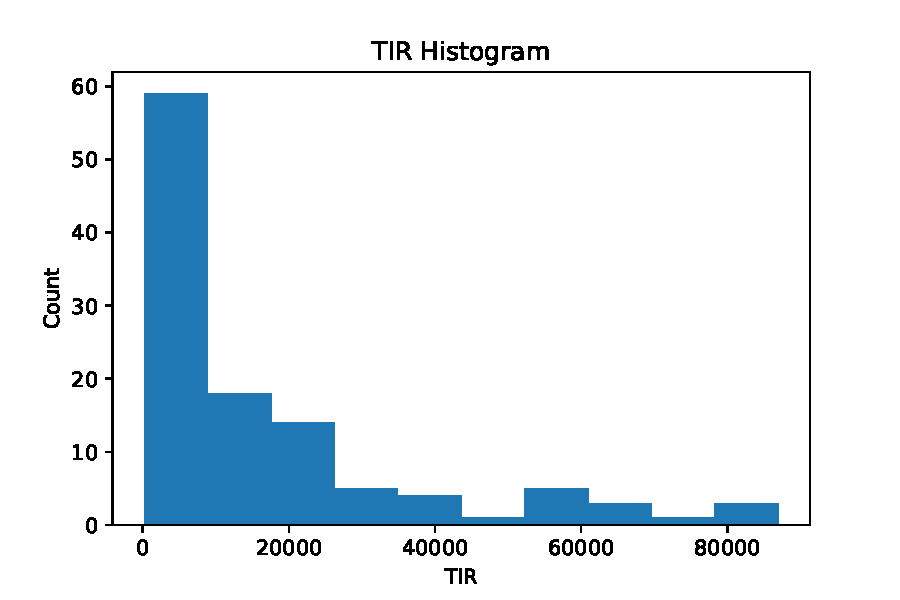
\includegraphics[scale=0.7]{plots/TIR_histogram.pdf}
    \caption{TIR Histogram.}
    \label{fig: TIR Histogram.}
\end{figure}

The RBS sequence is 20 bps, we focus on -8 to -13 bps and fix others as the same as the consensus sequence, i.e. TTTAAGA + NNNNNN + TATACAT. For each base, there are 4 possibilities: A, C, G, T. So totally the feature space is $4^6$ = 4096.

\subsection{Algorithms}

\subsubsection{Random sampling}

\subsubsection{Gaussian Process Upper Confidence Bound}

We use Gaussian Process Upper Confidence Bound (GPUCB)] algrithm \cite{srinivas2012information}, with sum of dot product kernel and spectrum kernel of sequences. The algorithm basically includes two parts:

\begin{enumerate}
    \item the Gaussian Process regression model, which predicts the label (TIR) and how uncertain we are about our prediction (confidence width); Since the sequences in provided data have the pattern that the core area is different from each other, and other areas are similar. So the kernel for Gaussian Process we are using is the sum of kernels, for core areas we use spectrum kernel with string as input directly, and for other areas we use one-hot encoding and dot product kernel for simplicity. 
    \item bandit algorithms (Upper Confidence Bound), which recommends sequences to test for next round.
\end{enumerate}

\section{Results}

\begin{enumerate}
    \item RMSE of predictions.
    
    \item Similarity of recommendations. 
    \begin{figure}[t]
    \centering
    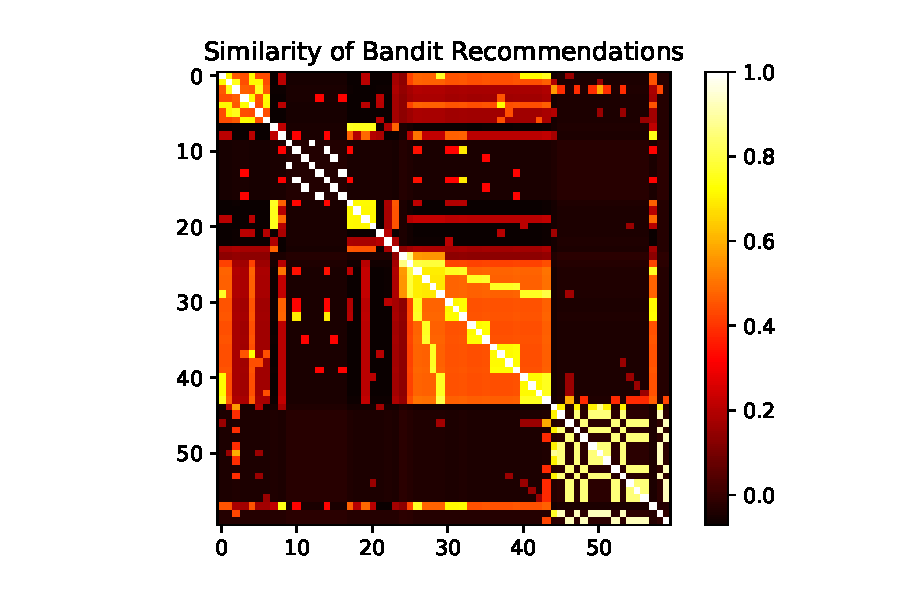
\includegraphics[scale=0.7]{plots/similarity_first_round_recommendation.pdf}
    \caption{TIR Histogram.}
    \label{fig: TIR Histogram.}
\end{figure}
\end{enumerate}{}

\section{Methods}

\newpage

\printbibliography
\end{document}
